\chapter{理论分析}
\label{chap:theory}
在这一章,我们将会对涉及到的理论与算法原理进行介绍。
\section{博弈树}
具有竞争或对抗性质的行为称为博弈行为。在这类行为中,参加斗争或竞争的各方各自具有不同的目标或利益。为了达到各自的目标和利益,各方必须考虑对手的各种可能的行动方案,并力图选取对自己最为有利或最为合理的方案。比如日常生活中的下棋,打牌等。博弈论就是研究博弈行为中斗争各方是否存在着最合理的行为方案,以及如何找到这个合理的行为方案的数学理论和方法\cite{gt}。
而博弈树是博弈理论中表达一个博弈中各种后续可能性的树。完整博弈树(Complete Game Tree)从代表某个博弈情景的起始节点出发,向下延展出若干层的子节点直到博弈结束。下一层的子节点是基于其父节点博弈行为所导致的可能性。博弈树中形成的叶节点代表各种游戏结束的可能情形,例如井字游戏(Tic-Tac-Toe)会有26,830个叶节点\cite{NAU1982257,allis1994searching}。


博弈树在人工智能应用领域占有重要地位,在博弈游戏中选择最佳动作的一种方法便是使用某种树搜索算法,结合类似于极小化极大算法的规则来修剪树,从而搜索整个博弈树。例如在井字游戏中计算机可以很快速地找到最佳解并做出决策,但是对于象棋、围棋这一类状态空间复杂的大型博弈游戏,受限于计算机性能遍历完整博弈树不太现实,因此对这类游戏通常会采用部分博弈树(partial game tree)来进行搜索。典型的部分博弈树通常是限制博弈树的层数,并剔除不佳的步法(例如自杀),一般而言搜索的层数越多,能走出较佳步法的机会也越高\cite{coin12162}。

\subsection{极小化极大算法}
极小化极大算法(Minimax)是人工智能领域常见的搜索算法,是一种找出失败的最大可能性中的最小值的算法,常用于棋类等由两方较量的游戏和程序,这类程序由两个游戏者轮流,每次执行一个步骤。该算法是一种零总和算法,即一方要在可选的选项中选择将其优势最大化的选择,而另一方则选择令对手优势最小化的方法\cite{ctt1r2gkx}。

\begin{figure}[htb]
    \centering
    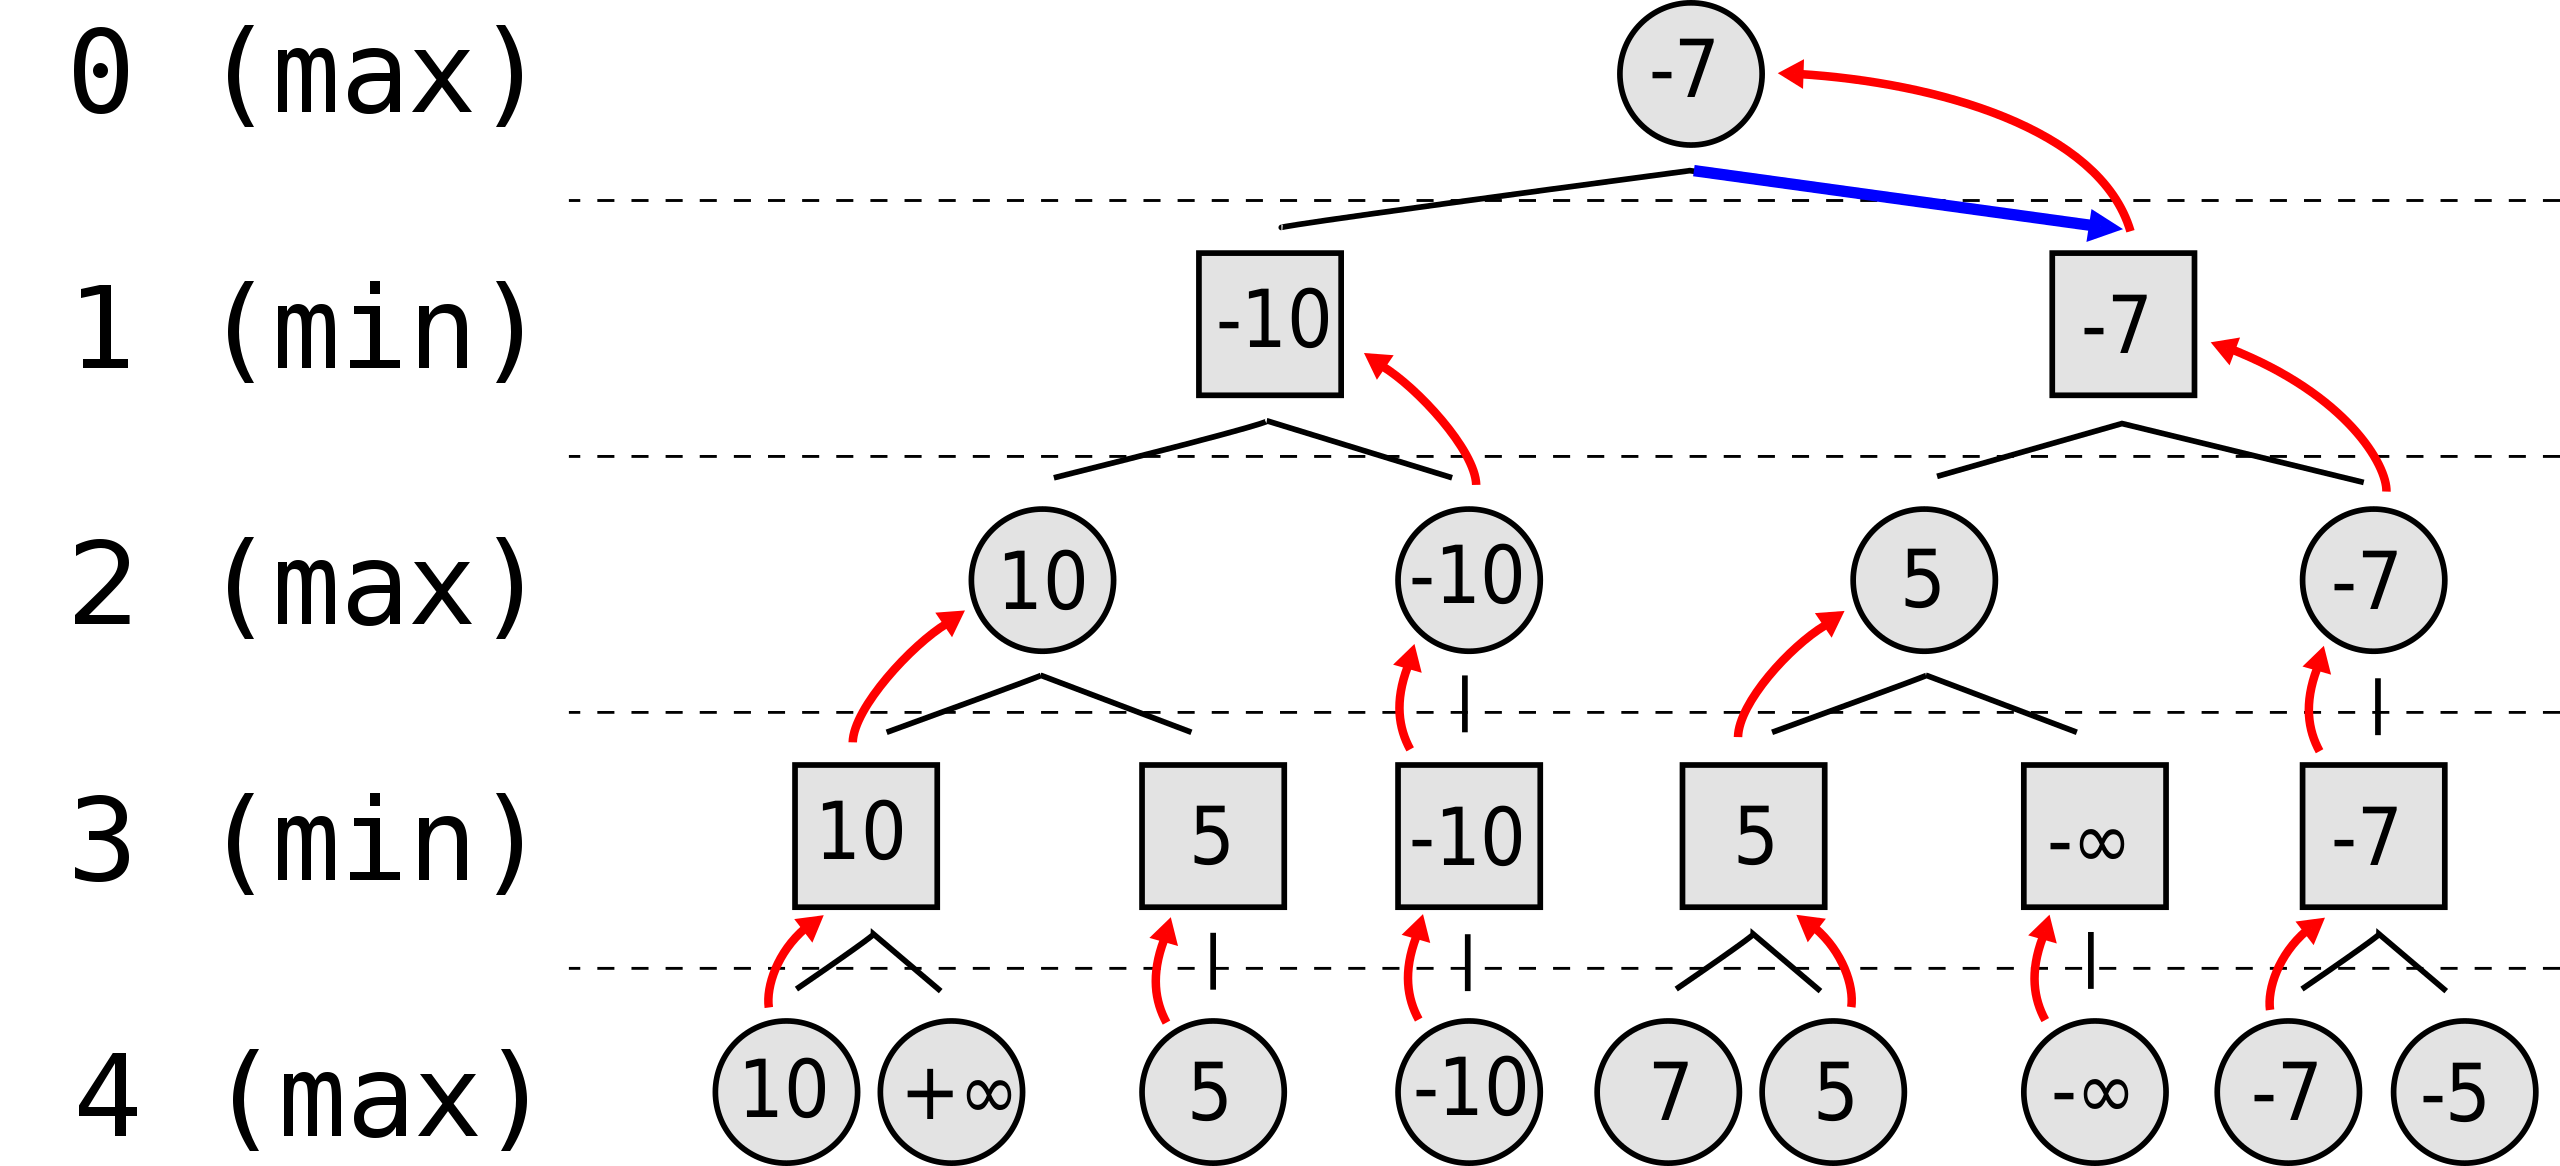
\includegraphics[width=0.6\textwidth]{Minimax.png}
    \caption[minimax]{%
      极小化极大算法搜索树例子\cite{wikiMinimax}%
      }
    \label{fig:minimax}
  \end{figure}

如图2.1所示,假设圆形代表当前选手,方形代表对手。当前选手需要将自己所得分数最大化,而对手则需要反其道行之。考虑第三层(Min层)对手在最左侧节点的决策,当前选手在第四层有得分为10或正无穷的行动选择,作为对手要做的是最小化这个分数,于是对手根据结果可以反推出应选择得分为10的行动。其余同理。
\subsection{Alpha-beta 剪枝}
在上一个小节中我们介绍了经典的极小化极大算法,对于一个具有复杂状态空间的游戏(象棋或围棋)来说,Minimax算法需要非常多层才能够完成。如果这个游戏每一步都有$n$个选择,那么在$x$步以后,将会有$n^x$个选择,也就是说具有指数级复杂度。在这种情况下,使用经典的极小化极大算法进行树搜索是不现实的。因此我们就需要采取剪枝来减少运算量,剪掉上述树状图的一些分支,从而减少运算量。

Alpha-beta剪枝用于裁剪搜索树中不需要搜索的节点。$\beta$值为可行解的最小上界(Min层通向root的路径上最好的选择),$\alpha$值为可行策略(解)的最大下界(Max层通向root的路径上最好的选择)。其在生成博弈树的同时计算评估各节点的$\alpha$值与$\beta$值, 并且根据评估出的值范围, 及时停止扩展那些已无必要再扩展的子节点,以提高运算速度。该算法和极小化极大算法所得结论相同,但剪去了不影响最终决定的分枝\cite{russell2010artificial}。
剪枝过程遵循$\alpha \le N \le \beta$,N为当前节点评估值。即:(1)当一个 Min 节点的 $\beta$值小于等于任何一个父节点的$\alpha$值时 ,剪掉该节点的所有子节点;(2)当一个 Max 节点的 $\alpha$值大于等于任何一个父节点的$\beta$值时 ,剪掉该节点的所有子节点。
我们用以下Minimax树(图2.1)作为例子,方块为Max节点,圆形为Min节点\cite{russell2010artificial}。
\begin{figure}[htb]
    \centering
    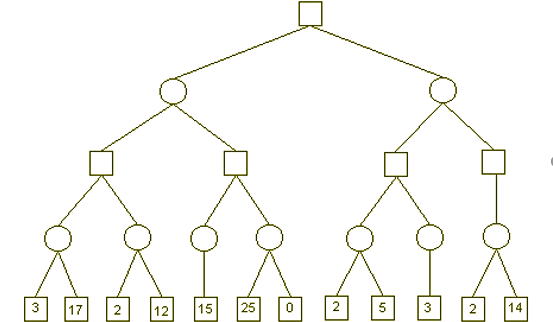
\includegraphics[width=0.6\textwidth]{abp1.PNG}
    \caption[abp]{%
    Alpha-beta剪枝初始状态\cite{russell2010artificial}%
      }
    \label{fig:abp}
  \end{figure}

其剪枝过程如图2.3所示。从左节点开始,

(1)当到达深度为4层处的第一个子节点时,在该状态上进行评估并获得值为3。将此节点值传递回上面的父Min节点。由于这是一个Min节点,因此该节点的Minimax值必须小于或等于3。换句话说,我们将该Min节点$\beta$值更改为3;

(2)接下来在深度为4层处遍历下一个子节点,并向父Min节点返回值17;

(3)由于父节点为Min节点,并且17大于3,因此将忽略返回17的子节点。 现在我们已经评估了这个Min节点的所有子节点,因此我们将$\beta$值返回到上面的Max节点。 Max节点的值将大于或等于3,因此我们将$\alpha$更改为3:

(4)遍历该Max节点的新Min子节点,并将当前的区间传递给子节点;

(5)搜索新Min子节点的子节点,第一个值为2并传递给Min父节点;

(6)父节点的值将小于或等于2,因此将其$\beta$值改为2;我们发现在此节点上找到解决方案路径的唯一方法是找到一个值大于3且小于2的子节点。由于这是不可能的,我们可以停止评估此节点的子节点,然后返回$\beta$值(也就是2)作为该节点的值。
回到父Max节点,其$\alpha$值已经是3,比2更具限制性,因此不要更改它。我们已经看到了此max节点的所有子节点,因此可以将其值设置为最终的$\alpha$值即为3。

\begin{figure}[htb]
    \centering
    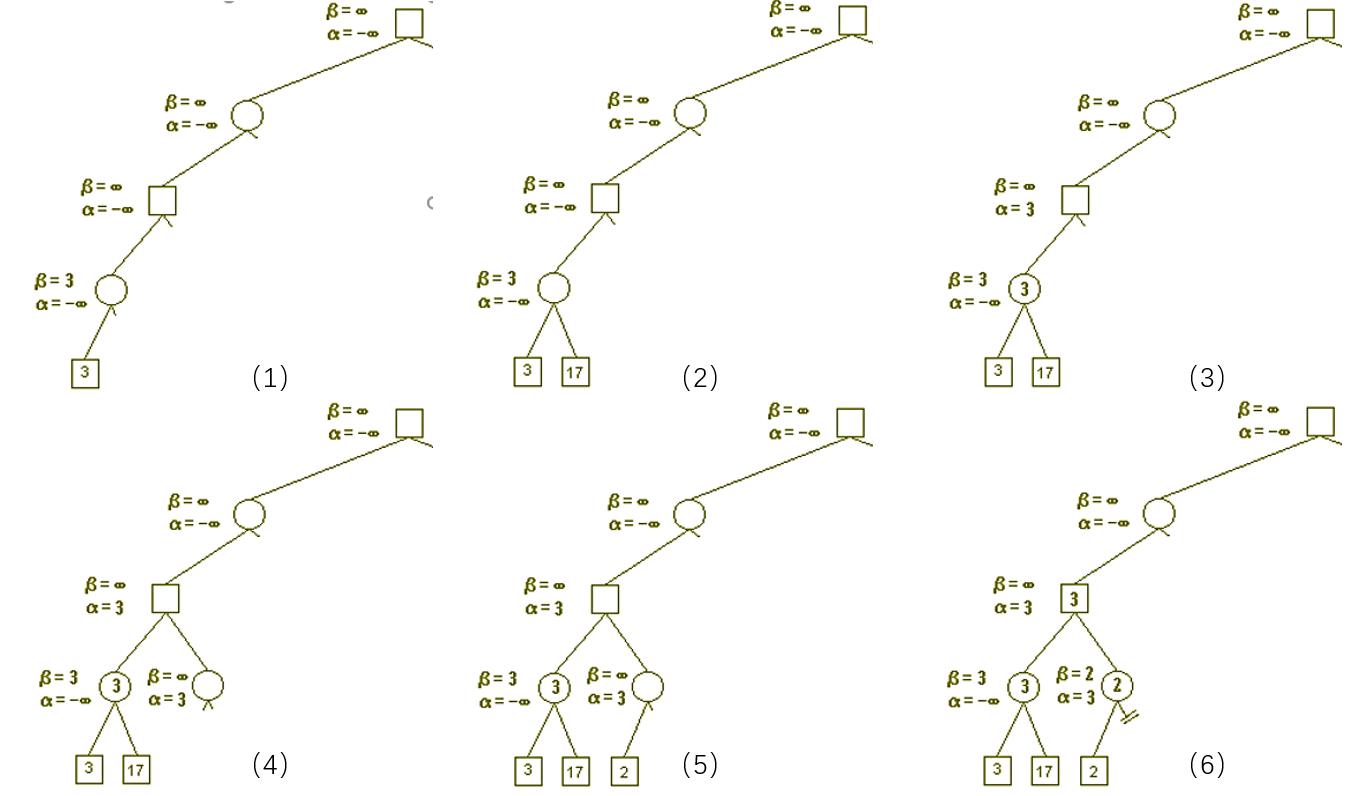
\includegraphics[width=0.9\textwidth]{abp2.PNG}
    \caption[abp2]{%
    Alpha-beta剪枝\cite{russell2010artificial}%
      }
    \label{fig:abp2}
  \end{figure}
\newpage
Alpha-beta剪枝是在极小化极大算法上的改进,减少搜索树的分枝,从而提升搜索深度。
若节点搜索顺序达到最优化或近似最优化(将最佳选择排在各节点首位),则同样时间内搜索深度可达极小化极大算法的两倍多\cite{KNUTH1975293abp}。但是对于较复杂的棋类游戏,若对AI的每一步有时间限制,Alpha-beta剪枝的搜索深度依然受到较大限制,在实际应用中往往采取3-4层,也有可能导致只能获得局部最优解。
除此之外,对手玩家一定会选择使自己最差的思路的先验假设,在真实情况下并不正确,因为无法确定对方的博弈策略是否和自己一致。如果对方做的策略不是最优,那么我方策略是最优的假设也不复存在。

\subsection{蒙特卡洛树搜索}
蒙特卡洛树搜索(Monte Carlo tree search,简称:MCTS)是一种启发式搜索算法,其在游戏树搜索的应用十分广泛\cite{10.1007/978-3-540-75538-8_7}。顾名思义,其设计思路是基于概率的:蒙特卡洛树搜索会多次模拟博弈过程,并尝试根据模拟结果预测最优的移动方案。这也与人类下棋时的思维模式符合:根据“棋感”在脑海里大致筛选出了几种最可能的走法,然后再想走了这几种走法之后对手最可能的走法,然后再想自己接下来最可能的走法。

蒙特卡洛树搜索的每个循环包括四个步骤\cite{RePEc:wsi:nmncxx:v:04:y:2008:i:03:n:s1793005708001094}:
(1)选择(Selection):从根节点开始,选择连续的子节点向下至叶子节点。选择子节点的方式一般采取上限置信区间算法(UCT)\cite{10.1007/11871842_29};
(2) 扩展(Expansion):创建一个或多个子节点并选取其中一个节点直到游戏结束;
(3)模拟(Simulation):在从选定的节点开始,用随机策略进行游戏,此过程又称为rollout;
(4) 反向传播(Backpropagation):使用随机游戏的结果,更新从选定节点到根节点的路径上的节点信息。
谷歌公司的AlphaGo/Zero体系中都使用了MCTS的架构并对其策略进行了改进与优化。

\begin{figure}[htb]
    \centering
    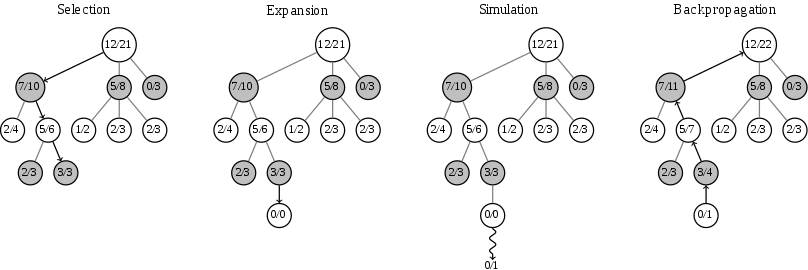
\includegraphics[width=0.9\textwidth]{mctswiki.png}
    \caption[mcts]{%
    蒙特卡洛树搜索的步骤,每一个节点的内容代表胜利次数/游戏次数\cite{RePEc:wsi:nmncxx:v:04:y:2008:i:03:n:s1793005708001094}%
      }
    \label{fig:mcts}
  \end{figure}
\newpage

\subsubsection{选择子节点的方式}
在蒙特卡洛树搜索中,可以将节点分为3类:

\begin{itemize}
    \item [(1)] 
    从未访问过:还没有评估过当前局势
    \item [(2)]
    未完全展开:被评估过至少一次,但是子节点(即下一步的局势)没有被全部访问过,可以进一步扩展
    \item [(3)]
    完全展开:子节点被全部访问过
\end{itemize}

搜索开始时,根节点的所有子节点都未被访问。选中第一个节点,第一个模拟过程就开始了。当初次访问节点的模拟结束后,其结果会反向传播至当前博弈树的根节点。模拟开始的节点被标注为已访问。
反向传播模拟结果的目的是更新反向传播路径上所有节点 $v$ 的总模拟奖励 $Q(v)$ 以及总访问次数 $N(v)$。在实践中,$Q(v)$是该节点胜利的次数,$N(v)$是该节点模拟的次数。胜利次数多的节点是较好的可利用候选(继续扩展可以维持胜率),而模拟次数少意味着该节点访问次数少,也可能因为尚未得到很好的探索而具有价值。
利用这两个节点属性构建树的置信上限(UCT)\cite{10.1007/11871842_29}在被访问节点中选择下一个要遍历的节点:
\begin{equation}
    UCT(v_{i},v) = \frac{Q(v_{i})}{N(v_{i})} + c\sqrt{\frac{log(N(v))}{N(v_{i})}}
\end{equation}
$c$为一个常数,用来平衡高胜率(加号前面)与低访问次数(加号后面),$v_{i}$为$v$的子节点。UCT值最大的节点就是蒙特卡洛树搜索遍历过程中选择的节点:其每次从根节点出发,每次选择己方 UCT 值最优的一个节点,向下搜索,直到找到一个未完全展开的节点,根据定义,未完全展开的节点一定有未访问的子节点,随机选择进行扩展。扩展会为刚刚选择的节点加上一个统计信息为$(Q(v)=0,N(v)=0)$的节点,然后进入下一步模拟。
在我们后续使用AlphaZero架构构建超级皇后AI时,模拟的步骤可以直接使用神经网络进行评估\cite{Silver1140,Silver2017,Silver2016}。

\section{卷积神经网络模型}
卷积神经网络(Convolutional Neural Network)是一个超级大的话题,我们不打算在此进行过度展开,仅进行少部分与棋类游戏AI相关的概念介绍,为后面方法设计部分打下理论基础。

卷积神经网络,也被称作CNN,是一种前馈神经网络\cite{SCHMIDHUBER201585},对于大型图像处理有出色表现\cite{NIPS2012_4824}。卷积神经网络由多个卷积层(Convolutional layers)和全连通层(Fully connected layers)组成,同时也包括关联权重(Weights)和池化层(Pooling layers)\cite{venkatesan2017convolutional}。
这一结构使得卷积神经网络能够利用输入数据的二维结构,卷积神经网络也因此在图像任务上能够给出更好的结果\cite{VALUEVA2020232}。其经典模型诸如深度残差网络(ResNet)\cite{resnet}等在诸多图像任务中发挥着重要作用。

那为何要在棋类游戏中引入卷积神经网络呢?在上一节中,我们提到过模拟的步骤可以直接使用神经网络进行评估,也就是说需要模拟才能获得的节点选择概率可以基于数据直接生成。神经网络非常适合基于大量数据产生概率,并且由于棋盘状态往往是二维结构,类似于图像,因此卷积神经网络便自然而然地被引入了\cite{Silver1140,Silver2017,Silver2016}。

\section{强化学习}
\subsection{马尔可夫决策过程与策略探索}
强化学习(Reinforcement Learning)也是一个历史悠久的超大话题,此处仅介绍部分重要概念。强化学习是除了监督学习和非监督学习之外的第三种基本机器学习方法,其强调如何基于环境而行动,以取得最大化的预期利益\cite{Sutton1998}。强化学习最典型的决策框架为马尔可夫决策过程(Markov Decision Processes,MDP)\cite{Bel}。
通常情况下MDP由四元组$(S,A,R,T)$定义:$S$为环境状态空间集合,$A$为智能体(agent)可选动作集合,$R(s,a)$函数返回在状态$s$中采取动作$a$所获得的报酬,$T(s^{'}|s,a)$为转移概率函数,指明了如果智能体在状态$s$中采取动作$a$,环境将转换为状态$s^{'}$的概率。
MDP问题的目标是找到使预期的未来奖励最大化的策略$\pi$。如果我们知道MDP的所有四元组元素是什么,我们就可以在实际执行操作之前直接计算出解决方案(奖励最大化策略)。MDP的一些经典规划算法包括值迭代,策略迭代等等\cite{Sutton1998}。但是强化学习与规划问题不同,智能体并不能知道MDP问题中的所有信息,无法直接算出解决方案。
具体而言,智能体不知道环境空间将如何响应其行动而发生变化(转移概率函数$T$未知),也不知道其行动会获得什么即时的报酬(奖励函数R)。相比于提前规划计算,智能体需要尝试在环境空间中采取行动,观察结果,并以某种方式从中找到一个好的策略。一般而言,有两种类型的算法可以帮助我们找到一个好策略\cite{rlbase}。

\paragraph{model-based算法}
让智能体从其对环境空间的观察中学习环境如何工作的模型是一个显而易见的方法。也就是说,如果agent当前处于状态$s_{1}$,采取行动$a_{1}$后,观察到环境以奖励$r_{2}$过渡到状态$s_{2}$,则此观察信息可通过监督学习改善转移概率函数$T(s_{2}|s_{1},a)$和奖励函数$R(s_{1},a_{1})$。
一旦agent对环境空间进行了充分的观察建模,就可以使用具有其学习模型的规划算法来寻找最优策略。 遵循此框架的算法是基于模型(model-based)的强化学习算法,需要知道状态之间的转移概率。
\paragraph{model-free算法}
顾名思义,model-free算法不依赖从环境空间中学习的模型。Q-learning\cite{vanHasselt2012}就是经典的model-free算法\cite{Sutton1998,tdgam,TechnicalNote},它通过选择当前状态下具有最高$Q$值的动作,直接在策略空间进行策略搜索并直接估算每个状态下每个动作的最佳Q值(“Q”这个字母在强化学习中表示一个动作的期望奖励),以找到可以从环境空间中获得更好回报的策略。
Q-learning步骤如下:(1)随机初始化$Q$值$Q(s,a)$;(2)根据当前$Q$值估计($Q(s,\cdot)$)在当前状态$s$下选择动作$a$;(3)采取动作$a$并观察结果状态$s^{'}$与奖励$r$;(4)使用贝尔曼方程\cite{dixit1990optimization}更新Q值:
\begin{equation}
  Q^{New}(s,a) = Q(s,a) + \alpha[R(s,a) + \gamma \max Q^{'}(s^{'},a^{'}) - Q(s,a)]
\end{equation}
$R(s,a)$为在状态$s$采取动作$a$的奖励,$\alpha$为学习率,$\gamma$为衰减系数,$\max Q^{'}(s^{'},a^{'})$为新状态$s^{'}$下可行动作的最高Q值。当$\gamma$数值越大时,agent便更加重视未来获得的长期奖励,$\gamma$数值越小时,agent更加短视只在乎目前可获得的奖励。
Q-learning没有从环境空间中学习模型,因此称为无模型(model-free)算法。

\subsection{策略迭代(Policy Iteration)\cite{Sutton1998}}
从一个初始化的策略出发,先进行策略评估(Policy Evaluation),然后改进策略(Policy Improvement),评估改进的策略,再进一步改进策略。经过不断迭代更新直到策略收敛,这种算法被称为\textbf{策略迭代},属于动态规划算法\cite{Sutton1998}。在棋类游戏AI强化学习中,此种思路经常被借鉴并发扬光大\cite{Silver1140,Silver2017,Silver2016}。
\paragraph{策略评估(Policy Evaluation)}
首先,我们考虑如何为任意策略$\pi$计算状态值函数$v_{\pi}$。设$G_{t}$为在$t$步的期望回报(expected return),$R_{t}$为在$t$步的奖励,$\gamma$同上为衰减率。则
\begin{equation}
  \begin{aligned}
  G_{t} & \doteq R_{t+1}+\gamma R_{t+2}+\gamma^{2} R_{t+3}+\gamma^{3} R_{t+4}+\cdots \\
  &=R_{t+1}+\gamma\left(R_{t+2}+\gamma R_{t+3}+\gamma^{2} R_{t+4}+\cdots\right) \\
  &=R_{t+1}+\gamma G_{t+1}
  \end{aligned}
\end{equation}
\begin{equation}
  \begin{aligned}
  v_{\pi}(s) & \doteq \mathbb{E}_{\pi}\left[G_{t} \mid S_{t}=s\right] \\
  &=\mathbb{E}_{\pi}\left[R_{t+1}+\gamma G_{t+1} \mid S_{t}=s\right] \\
  &=\mathbb{E}_{\pi}\left[R_{t+1}+\gamma v_{\pi}\left(S_{t+1}\right) \mid S_{t}=s\right] \\
  &=\sum_{a} \pi(a \mid s) \sum_{s^{\prime}, r} p\left(s^{\prime}, r \mid s, a\right)\left[r+\gamma v_{\pi}\left(s^{\prime}\right)\right],
  \end{aligned}
\end{equation}
$\pi(a|s)$是在策略为$\pi$时,在状态$s$下采取动作$a$的概率。迭代求解方法最适合式(2.4),考虑一系列近似值函数$v_{0},v_{1},v_{2}\dots$,任选$v_{0}$进行初始估计。接下来的每个近似估计都会使用$v_{\pi}$贝尔曼方程\cite{dixit1990optimization}进行迭代更新:
\begin{equation}
  \begin{aligned}
  v_{k+1}(s) & \doteq \mathbb{E}_{\pi}\left[R_{t+1}+\gamma v_{k}\left(S_{t+1}\right) \mid S_{t}=s\right] \\
  &=\sum_{a} \pi(a \mid s) \sum_{s^{\prime}, r} p\left(s^{\prime}, r \mid s, a\right)\left[r+\gamma v_{k}\left(s^{\prime}\right)\right]
  \end{aligned}
\end{equation}
序列$\{v_{k}\}$在$k$趋近于$\infty$时是收敛的\cite{kamien2013dynamic}。此算法被称为迭代策略评估\cite{Sutton1998}。
\begin{algorithm}[htb]
  \caption{迭代策略评估,使$V\approx v_{\pi} $}
  \begin{algorithmic}[1]
    \Require $\pi$ ,待评估的策略;$\theta$,用于调整预测精度的阈值
    \Ensure 评估结束的策略
    \State 随机初始化$V(s)$,避开终结状态;
    \Repeat
    \State $\Delta\Leftarrow 0$;
    \Loop 对于每个状态$s$:
    \State $v \leftarrow V(s)$;
    \State $V(s) \leftarrow \sum_{a} \pi(a \mid s) \sum_{s^{\prime}, r} p\left(s^{\prime}, r \mid s, a\right)\left[r+\gamma V\left(s^{\prime}\right)\right]$;
    \State $\Delta \leftarrow \max (\Delta,|v-V(s)|)$;
    \EndLoop
    \Until{直到 $\Delta \le \theta$}
  \end{algorithmic}
\end{algorithm}

\paragraph{策略提升(Policy Improvement)}
计算策略值函数的目的是为了寻找更好的策略。假设我们已经确定了任意决定性策略$\pi$的值函数$v_{\pi}$,但是在某些状态下采取新策略获得的收益可能更大,因此我们需要对切换到新策略是好是坏进行判断。
我们可以考虑在状态$s$下选择动作$a$并遵守当前策略。这样做的值可以表示为:
\begin{equation}
  \begin{aligned}
  q_{\pi}(s, a) & \doteq \mathbb{E}\left[R_{t+1}+\gamma v_{\pi}\left(S_{t+1}\right) \mid S_{t}=s, A_{t}=a\right] \\
  &=\sum_{s^{\prime}, r} p\left(s^{\prime}, r \mid s, a\right)\left[r+\gamma v_{\pi}\left(s^{\prime}\right)\right]
  \end{aligned}
\end{equation}
如果此值大于$v_{\pi}(s)$,说明最后获得的新策略从整体上更优。因此我们设$\pi$与$\pi^{'}$为任意一对决定性策略,当其满足$q_{\pi}\left(s, \pi^{\prime}(s)\right) \geq v_{\pi}(s)$时,策略$\pi^{'}$一点至少与策略$\pi$一样好,
\begin{equation}
  \begin{aligned}
  v_{\pi}(s) & \leq q_{\pi}\left(s, \pi^{\prime}(s)\right) \\
  &=\mathbb{E}\left[R_{t+1}+\gamma v_{\pi}\left(S_{t+1}\right) \mid S_{t}=s, A_{t}=\pi^{\prime}(s)\right] \\
  &=\mathbb{E}_{\pi^{\prime}}\left[R_{t+1}+\gamma v_{\pi}\left(S_{t+1}\right) \mid S_{t}=s\right] \\
  & \leq \mathbb{E}_{\pi^{\prime}}\left[R_{t+1}+\gamma q_{\pi}\left(S_{t+1}, \pi^{\prime}\left(S_{t+1}\right)\right) \mid S_{t}=s\right] \\
  &=\mathbb{E}_{\pi^{\prime}}\left[R_{t+1}+\gamma \mathbb{E}\left[R_{t+2}+\gamma v_{\pi}\left(S_{t+2}\right) \mid S_{t+1}, A_{t+1}=\pi^{\prime}\left(S_{t+1}\right)\right] \mid S_{t}=s\right] \\
  &=\mathbb{E}_{\pi^{\prime}}\left[R_{t+1}+\gamma R_{t+2}+\gamma^{2} v_{\pi}\left(S_{t+2}\right) \mid S_{t}=s\right] \\
  & \leq \mathbb{E}_{\pi^{\prime}}\left[R_{t+1}+\gamma R_{t+2}+\gamma^{2} R_{t+3}+\gamma^{3} v_{\pi}\left(S_{t+3}\right) \mid S_{t}=s\right] \\
  & \vdots \\
  & \leq \mathbb{E}_{\pi^{\prime}}\left[R_{t+1}+\gamma R_{t+2}+\gamma^{2} R_{t+3}+\gamma^{3} R_{t+4}+\cdots \mid S_{t}=s\right] \\
  &=v_{\pi^{\prime}}(s) .
  \end{aligned}
\end{equation}
上述不等式也意味着$v_{\pi^{\prime}}(s) \geq v_{\pi}(s)$,即更好的策略一定可以获得更大奖励。因此我们可以获得新的策略函数:
\begin{equation}
  \begin{aligned}
  \pi^{\prime}(s) & \doteq \underset{a}{\arg \max } q_{\pi}(s, a) \\
  &=\underset{a}{\arg \max } \mathbb{E}\left[R_{t+1}+\gamma v_{\pi}\left(S_{t+1}\right) \mid S_{t}=s, A_{t}=a\right] \\
  &=\underset{a}{\arg \max } \sum_{s^{\prime}, r} p\left(s^{\prime}, r \mid s, a\right)\left[r+\gamma v_{\pi}\left(s^{\prime}\right)\right]
  \end{aligned}
\end{equation}

\paragraph{策略迭代(Policy Iteration)}
当策略$\pi$通过上述步骤得到提升产生了新策略$\pi_{'}$,我们可以计算$v_{\pi^{'}}$并再次利用新的值函数得到更好的策略$\pi^{''}$如下所示:
\begin{equation}
  \pi_{0} \stackrel{\mathrm{Evaluation}}{\longrightarrow} v_{\pi_{0}} \stackrel{\mathrm{Improvement}}{\longrightarrow} \pi_{1} \stackrel{\mathrm{Evaluation}}{\longrightarrow} v_{\pi_{1}} \stackrel{\mathrm{Improvement}}{\longrightarrow} \pi_{2} \stackrel{\mathrm{Evaluation}}{\longrightarrow} \cdots \stackrel{\mathrm{Improvement}}{\longrightarrow} \pi_{*} \stackrel{\mathrm{Evaluation}}{\longrightarrow} v_{*}
\end{equation}
策略迭代的整体算法步骤如下。
\begin{algorithm}[htb]
  \caption{策略迭代算法,使$\pi \approx \pi_{*} $}
  \begin{algorithmic}
    \State 1.随机初始化$V(s)$与$\pi(s)$;
    \State 2.策略评估(迭代策略评估算法;
    \State 3.策略提升:
    \State $stable-policy \leftarrow True$
    \For{each $s\in\textbf{S}$}
    \State $当前动作\longleftarrow\pi(s)$
    \State $\pi(s) \leftarrow \arg \max _{a} \sum_{s^{\prime}, r} p\left(s^{\prime}, r \mid s, a\right)\left[r+\gamma V\left(s^{\prime}\right)\right]$
    \State 如果当前动作不等于$\pi(s)$,那么 $stable-policy \leftarrow False$
    \EndFor
    \State 如果$stable-policy = True$,则停止并返回$\pi \approx \pi_{*} $与$V\approx v_{\pi} $;否则返回步骤2
  \end{algorithmic}
\end{algorithm}

